\documentclass[a4paper]{article}
\title{\textcolor{red}{Workshop on Public Key Infrastructure and Red Hat Certificate System}}
\author{Niranjan M.R, Huzaifa Sidhpurwala, Asha Akkiangady}
\date{}
\usepackage{color}
\usepackage{graphics}
\usepackage{graphicx,subfig}
\begin{document}
\maketitle
\tableofcontents
\section{Introduction to Public Key Cryptography}
Before we start discussing about public key cryptography, we will in general discuss about how system communicate
and what are the various threat models that are associated with the communication medium and what are the tools to 
overcome them.

\textbf{Example1:}
The most common protocol used to communicate between 2 systems is TCP/IP. TCP/IP allows information to be sent 
from one system to another system directly or through many intermediate systems.

Below are some of the threat models associated with above communcation:
\begin{itemize}
    \item \textbf{Eavesdropping:}
        
        Information remains intact, But it's privacy is compromised, For example: some one could learn credit card number, record a sensitive conversation or intercept a
        classified information.
    \item \textbf{Tampering:}

        Information in transit is changed or replaced and then sent to the recipient. For example: Some one could alter an order of goods or change a persons resume.
    \item \textbf{Impersonation:}

        Information passes to a person who poses as intended recipient. Impersonation can take 2 forms:
    \begin{itemize}
        \item \textbf{Spoofing:}

            A person can pretend to be someone else, For example, a person can pretend to have email address \textit{joe@example.net}, 
            or computer can identify itself as a site called www.example.net, when it is not. This type of impersonation is called spoofing.
        \item \textbf{Misrepresentation:}

            A person or organization can misrepresent itself, For example, suppose the site \textit{www.example.net} pretends to be a 
            furniture store when it's just a site which accepts payments but never sends any goods.
    \end{itemize}
\end{itemize}
\textbf{Example2:}
Consider Alice , Bob and attacker are the parties , where alice and bob want to communicate to each other and Attacker is a threat to the communication.

\begin{itemize}
    \item Alice can send a postcard to bob to communicate, but this method is very weak as any random eavesdropper could read the postcard.
    \item Alice could write a letter and put in an envelope and send it to bob, but the attacker could open the envelope and read the letter, 
        both confidentiality and integrity of the message is lost.
    \item Alice could seal the envelope with wax , but this method too is inefficient as Attacker could read the letter and seal it as it is 
        without bob knowing that it was read by attacker
    \item Alice could write a letter and put it in a safe which has 2 keys and send one key before to Bob , and send the safe across to bob, 
        this ensures confidentiality, integrity but practically this is not implementable. Considering the number of 
        messages that has to be transferred , it's impractical to implement the mail safe method.
\end{itemize}

To mitigate above threat models, we will look in to cryptology as one of the tools of the trade. 

\textbf{Cryptology:} Cryptology is the theory of designing the various algorithms we use to provide security

\textbf{Cryptography:} Cryptography is the study of using these algorithms to secure systems and protocols.
\subsection{Encryption}
An encryption algorithm takes some data(called plaintext) and converts it to cipher-text under control of a key. 
cipher text contains random data which makes no sense without the key.  

A key is a short random string (8-24 bytes): 

\begin{picture}(10,10)(10,10)
    \put(40,1){\framebox(55,8){Plain Text}} 
    \put(102,10){\tiny Encryption}
    \put(102,4){\vector(1,0){30}}
    \put(140,1){\framebox(55,8){Cipher Text}} 
    \put(200,10){\tiny Decryption}
    \put(200,4){\vector(1,0){30}}
    \put(240,1){\framebox(55,8){Plain Text}} 
\end{picture}
\linebreak

When a message is encrypted and received , we cannot say if it's not tampered with. An encryption is strong when 
it can determine the number of possible keys. The attacker tries each key one at a time until he finds a key that 
produces a plausible decryption. The security of the algorithm should solely depend on the secrecy of the key. 
The algorithm should not need to be secret.

If the attacker knows the plaintext corresponding to the ciphertext it's called \textit{``known plaintext attack''} .

An attack where attacker doesn't know the plaintext , it's called \textit{``ciphertext-only attack''}.
\textit{Ex:} If the attacker knows that plaintext is ASCII , so any decryption which uses non-ascii characters must be using the wrong key.
\subsubsection{Symmetric Encryption}
When Sender and recipient share the same key(which must be kept secret) is referred to as \textit{Symmetric Key Cryptograph} or also
referred to as \textit{Secret Key Cryptography} as opposed to \textit{Public Key Cryptography}citation required?.
\begin{figure}[h]
    \centering
    \includegraphics[width=50mm]{symmetric.png}
    \caption{Symmetric Encryption}
\end{figure}
\subsubsection{Assymetric Encryption}
\begin{itemize}
    \item First started in stanford university by Whitfield Diffie and Martin Hellman
    \item The most commonly used implementation of PKC are based on algorithm based on algorithm patented by RSA data security.
    \item Each public key is published \& private key is kept secret. Data encrypted with public key can be decrypted only with private key.
    \item In general, to send encrypted data to someone, we encrypt with public key \& the person encrypt receiving the 
        encrypted data decrypts with private key
    \item Compared to symmetric key encryption, public key encryption requires more computation \& therefore not always appropriate for large amounts of data
    \item It is possible to use public-key encryption to send a symmetric key, which can then be used to encrypt additional data.
        \begin{figure}[h]
            \centering
            \includegraphics[width=80mm]{assymetric.png}
            \caption{Assymetric Encryption}
        \end{figure}
    \item Reverse of the above figure also happens i.e. encrypt with private key and decrypt with public-key. But not useful for sensitive information
        \begin{figure}[h]
        \centering
        \includegraphics[width=80mm]{digitalsignature.png}
        \caption{Digital Signature}
        \end{figure}
    \item There's a problem with the above method, how would the parties get each other's public-key ? 
        If we send the keys through electronically, then the attacker an tamper, while they are in transit to the receiver.
    \item When the 2 parties want to communicate, the attacker can intercept the keys \& instead send his own key to each other, 
        thus each party encrypts to him and \& he re-encrypts it to the real recipient. 
        This is called \textit{man-in-the-middle attack}
        \begin{figure}[ht!]
            \centering
            \includegraphics[width=50mm]{mitm.png}
            \caption{Man-in-the-middle attack}
        \end{figure}
\end{itemize}
\subsection{Message Digest}
A message digest is simply a function that takes as an input an arbitrary message and outputs a fixed length string 
which is characteristic of the message. The important property here is irreversibility.  
It's extremely difficult to compute a message from the given digest. 
Property of the message digest: 
\begin{itemize}
    \item For a digest to be secure, it must be difficult to generate any of the message that digests to the same value. 
        You have to search a message space of proportional size of the digest in order to find a matching message text
    \item It should be difficult to produce 2 messages M and M' such that they have the same digest. 
        This property is called collision-resistance. It turns out that the strength of any message digest 
        against finding collision is only half the size of the digest., so a 128-bit digest is only 64 bits strong against collisions.
\end{itemize}
\subsubsection{Message Authentication Code}
Consider \textit{Alice} and \textit{Bob} share a key and Alice wants to send a message to \textit{Bob}. The message can be encrypted, 
and send it across to \textit{Bob}, but we are not sure that the encrypted message would be tampered and also not sure 
if \textit{Alice} was the one who sent the encrypted message.  So we use a new tool called \textit{MAC} . \textit{MAC} is a digest algorithm,
but with a key, So the MAC is dependent on both the key and the message being MACed.
\subsection{Protocols}
\subsection{Exercises}
\section{Introduction to Public Key Infrastructure}
Below is a simplified architectural model of Public Key Infrastructure using X.509 (PKIX) Specifications
\begin{figure}[ht!]
    \centering
    \includegraphics[width=70mm]{pki-architectural-model.png}
    \caption{PKI Architectural Model}
\end{figure}
\subsection{Common Terms used in PKI}
\begin{itemize}
    \item \underline{End Entiy}: User of the PKI certificates and/or end user system that is the subject of a certificate
    \item \underline{CA}: Certificate Authority
    \item \underline{RA}: Registration Authority, Optional System to which CA delegates certain management functions
    \item \underline{CRL issuers}: A system that generates CRL
    \item \underline{repository}: a system or collection of distributed systems that stores certificates and CRLs and services as a means of distributing these certificates and CRLs to end entities
\end{itemize}
\subsection{Detailed look on certificate/CRL}
    \subsubsection {Certificates}
        \begin{itemize}
            \item Certificates are data structures that bind public key values to the subject. This binding is asserted by a trusted Certificate Authority.
            \item X.509 defines the standard certificate format and v3 is the latest version.
            \item Internet Privacy Enhanced Mail(PEM) RFC 1421 and 1422 also include specifications for PKI based on X.509 certs. 
            \item Types of Certificates:
                \begin{itemize}
                    \item End-Entity
                    \item CA
                \end{itemize}
            \item RFC 1422 defines hierarchial structure  of CA's and there are three types of PEM CA
                \begin{itemize}
                    \item IPRA: Internet Policy Registration Authority , acts as Root of Certificate authority. IPRA operates under Internet Society Organization
                    \item PCA: Policy Certificae Authority ,(Verisign, Digicert, etc) signed by IPRA
                    \item CA: Certificate Authorities signed by PCA (Organizational CA's)
                \end{itemize}
            \item Policies used by CA:
                \begin{itemize}
                    \item IPRA certifies only PCA and not CA's or users cert
                    \item IPRA will make sure that the DN of the PCA is unique and will not certificate PCA's with similar DN
                    \item Certificates should not be issued to distinct entities under the same distinguished Name. 
                    \item IPRA should not certifiy two PCA's with same DN
                    \item PCA's should not certify two CA's with same DN
                    \item CA's are expected to sign certificates only if the subject DN in the
                        certificates is subordinate to the issuer CA DN.
                \end{itemize}
            \item Types of Certificate Authorities
                \begin{itemize}
                    \item Cross-Certs: Where Issuer and Subject are different
                    \item Self-Issue: Where Issuer and Subject are same
                        \begin{itemize}
                            \item Self-Signed: Where key bound in to the certificate is same as the key used to sgin the certificate
                        \end{itemize}
                \end{itemize}
        \end{itemize}
    \subsubsection{Basic Certificate Fields}
        \begin{itemize}
            \item Version:
                \begin{itemize}
                    \item Describes the version of encoded certificate.
                    \item if extensions are used: \textbf{0x2(3)}
                    \item if extensions are not used but UniqueIdentifier is used: \textbf{0x1(2)}
                    \item if only basic fields are there: \textbf{0x0(1)}
                \end{itemize}
                \begin{itemize}
                    \item Values: \textbf{0x2(3), 0x1(2), 0x0(1)}
                \end{itemize}
            \item Serial Number:
                \begin{itemize}
                    \item Positive integer assigned by CA to each certificate
                    \item It must be unique for each Certificate given by CA
                    \item Can contain long integers (up to 20 Octets)
                \end{itemize}
                \begin{itemize}
                    \item Values: Integers: 
                    \begin{itemize}
                        \item \textbf{16694152257348400000}
                        \item \textbf{0xe7ad8b07558a1727}
                        \item \textbf{cd:ba:7f:56:f0:df:e4:bc:54:fe:22:ac:b3:72:aa:55}
                    \end{itemize}
                \end{itemize}
            \item Signature:
                \begin{itemize}
                    \item Algorithm used by \textbf{CA} to sign the certificate
                    \item Value:
                        \begin{itemize}
                            \item \textbf{md2WithRSAEncryption}
                            \item \textbf{sha1WithRSAEncryption}
                        \end{itemize}
                \end{itemize}
            \item Issuer:
                \begin{itemize}
                    \item Identifies the entity that has signed and issued the certificate
                    \item \textbf{MUST} contain non-empty Distinguished Names
                    \item Names should confirm to X.501 standard
                    \item Generally contains Country, Organization, Common name, SerialNumber,
                        province, State, title, Surname, Generation Qualifier(Jr, Sr).
                    \item Values:
                    \begin{itemize}
                        \item \textbf{C=US, O=VeriSign, Inc., OU=Class 1 Public Primary Certification Authority}
                        \item \textbf{C=DE, ST=Bayern, L=Muenchen, O=Whatever it is, CN=IO::Socket::SSL Demo CA}
                        \item \textbf{C=US, O=VeriSign, Inc., OU=Class 1 Public Primary Certification Authority}
                    \end{itemize}
                \end{itemize}
            \item Validity:
                \begin{itemize}
                    \item The time interval during which the CA warrants that it will maintain status of the certificate
                    \item Consists sequence of 2 dates
                        \begin{itemize}
                            \item Date on which certificate validity begins
                            \item Date on which certificate validity ends
                        \end{itemize}
                    \item Validity period of a certificate is period from notBefore to notAfter(inclusive)
                    \item Values:
                        \begin{itemize}
                            \item \textbf{Not Before: Jan 29 00:00:00 1996 GMT}
                            \item \textbf{Not After : Aug  1 23:59:59 2028 GMT}
                            \item Special Note:
                                \begin{itemize}
                                    \item Devices are given certificates where there is no expiration date
                                    \item Value:
                                    \item Certificate is to be used for entire lifetime of the device \textbf{ Not After: 99991231235959Z.(represented in Generalized Time)}
                                \end{itemize}
                        \end{itemize}
                    \end{itemize}
            \item Subject:
                \begin{itemize}
                    \item Identifies the entry associated with public key stored in the subject public key field 
                    \item If the subject is CA then it should be populated with same data as issuer 
                    \item Names should confirm to X.501
                    \item Values:
                        \begin{itemize}
                            \item \textbf{C=US, ST=North Carolina, O=Fedora Project, OU=Fedora User Cert, CN=mrniranjan/emailAddress=niranjan@ashoo.in}
                        \end{itemize}
                \end{itemize}
            \item Subject Public key Info:
                \begin{itemize}
                    \item This field is used to carry public key and identify the algorithm with which the key is used (RSA, DSA)
                    \item Supported Cryptographic Algorithms:
                        \begin{itemize}
                            \item \textbf{Rivest-Shamir-Adelman (RSA)}
                            \item \textbf{Digital Signature Algorithm (DSA)}
                            \item \textbf{Diffie-Hellman (DH)}
                            \item \textbf{Elliptic Curve Digital Signature Algorithm (ECDSA)}
                            \item \textbf{Key Encryption Algorithm (KEA)}
                            \item \textbf{Elliptic Curve Diffie-Hellman (ECDH)}
                        \end{itemize}
                \end{itemize}
            \end{itemize}
    \subsubsection{Extensions}
        \begin{itemize}
            \item This field only appears in v3 Certs
            \item This contains sequence of one or more Certificate Extensions 
            \item Extensions provides method for associating additional attributes with public keys
            \item Managing relationship between CA's
            \item Can carry private extensions to carry information unique to their community
            \item Each Extension is either Critical / Non Critical
            \item Each Extension includes OID and ASN.1 DER  (OCTET)
                \begin{itemize}
                    \item Example: DE:65:01:16:19:2E:51:E0:9A:51:1A:37:50:94:7D:39:29:2A:42:2C
                \end{itemize}
            \item There cannot be duplicates of Extensions
            \item Default CRITICAL value is false
            \item If the Certificate is CA , then they should have below Extensions
                \begin{itemize}
                    \item Basic Key Identifier
                    \item Authoritative key Identifier
                    \item Basic Constraints
                \end{itemize}
        \end{itemize}
        \begin{itemize}
            \item \textbf{Authority Key Identifier:}
                \begin{itemize}
                    \item Provides a means of identifying the public key corresponding to the private key used to sign the certificate
                    \item This is required if the issuer has multiple signing keys 
                    \item If the CA certificate is self signed Authority key identifier is skipped
                    \item Values:
                        \begin{itemize}
                            \item \textbf{keyid:48:E6:68:F9:2B:D2:B2:95:D7:47:D8:23:20:10:4F:33:98:90:9F:D4}
                        \end{itemize}
                \end{itemize}
            \item \textbf{Subject Key Identifier:}
                \begin{itemize}
                    \item Provides a means of identifying certificates that contain a particular public key
                    \item This extension is must for CA certificates
                    \item The value placed in this is same as Authority Key Identifier
                    \item For End-entity Certificates, this extension provides a means for identifying certificates containing particular key used in application
                    \item Value:
                        \begin{itemize}
                            \item \textbf{48:E6:68:F9:2B:D2:B2:95:D7:47:D8:23:20:10:4F:33:98:90:9F:D4}
                        \end{itemize}
                \end{itemize}
            \item \textbf{Key Usage:}
                \begin{itemize}
                    \item Defines the purpose of the key contained in the certificate 
                    \item This extension is used to restrict the usage of the key to be used for purpose 
                        other than what is defined in Key Usage
                    \begin{itemize}
                        \item \textbf{digitalSignature}
                            \begin{itemize}
                                \item Public key should be used only to verify signatures on objects other than Public key certificates/CRL
                            \end{itemize}
                        \item \textbf{nonRepudiation/contentCommitment}
                            \begin{itemize}
                                \item subject Public key is used to verify digital signatures other than signatures on public key(CRL)
                                \item used to provide nonRepudiation Service that protects against signing entity falsely denying any public action
                            \end{itemize}
                        \item \textbf{keyEncipherment}
                            \begin{itemize}
                                \item Public key is used for enciphering private key or secret keys , 
                                \item Is used for encrypting symmetric content-decryption key or an assymetric private key
                            \end{itemize}
                        \item \textbf{dataEncipherment}
                            \begin{itemize}
                                \item is used for enciphering the raw data without the use any cipher  (very rarely used)
                            \end{itemize}
                        \item \textbf{keyAgreement}
                            \begin{itemize}
                                \item is used for key Agreement, 
                                \item when used Deffie-Hellman key is to be used for key management
                            \end{itemize}
                        \item \textbf{keyCertSign}
                            \begin{itemize}
                                \item Public key is used for verifying the signatures on public keys , if this is true then 
                            \end{itemize}
                        \item \textbf{cRLSign}
                            \begin{itemize}
                                \item when the subject public key is used for verifying signatures of CRL 
                            \end{itemize}
                        \item \textbf{encipherOnly}
                            \begin{itemize}
                                \item subject's public key may be used only for enciphering data while performing key agreement
                            \end{itemize}
                        \item \textbf{decipherOnly}
                            \begin{itemize}
                                \item subject's public key may be used only for deciphering data while performing key agreement
                            \end{itemize}
                        \item Important Note:
                            \begin{itemize}
                                \item \begin{figure}[ht!]
                                    \centering
                                    \includegraphics[width=70mm]{KeyUsage1.png}
                                    \caption{Key Usage restrictions}
                                \end{figure}
                            \end{itemize}
                    \end{itemize}
                \end{itemize}
            \item \textbf{Certificate Policies}
                \begin{itemize}
                    \item Contains sequence of one or more policy information terms each of which consits of
                        OID, optional Queries
                    \item OID Should not appear more than once
                    \item for End-entity policy information terms indicate the policy under which the certificate
                        has been issued and purposes for which the certificate must be used
                    \item For CA the policy limits the policies for certificate paths that include this certificate
                    \item if CA does not want to limit the set of policies for certification paths then it may assert
                        \textbf{anyPolicy} with value \textbf{2.5.29.32.0}
                    \item Policy Qualifiers:
                        \begin{itemize}
                            \item CPSNotice: Points URL to \textit{certificate practice statement} document that describes
                                the policy under which the subject was issued
                            \item userNotice: text that describes the policy(not more than 200 characters)
                        \end{itemize}
                \end{itemize}
            \item \textbf{Policy Mappings}
                \begin{itemize}
                    \item This extension is used by CA certificates 
                    \item Lists one or more pairs of OID, which indicate that the corresponding policies 
                        of one CA are equivalent to policies of another CA [used in context of Cross pair certificates]
                    \item \textbf{OID: 2.5.29.33}
                \end{itemize}
            \item \textbf{Subject Alternative Name}
                \begin{itemize}
                    \item Allows alternate names to be bound to subject of the certificate. 
                    \item The names specified in subjectAltName may be included in addition to
                        or in place of the identity in the subject field of the certificate
                    \item Defined subject names used:
                        \begin{itemize}
                            \item rfc822Name:       IA5String
                            \item otherName:        OtherName
                            \item dNSName:          IA5String
                            \item directoryName:    Name
                            \item URI:              IA5string
                            \item iPAddress:        OCTET String
                            \item UniformResourceIdentifier: IA5String
                        \end{itemize}
                \end{itemize}
            \item \textbf{Issuer Alternative Name}
                \begin{itemize}
                    \item Allows alternate names to be bound to certificate issuer
                    \item Issuer alternative names are not processed as part of certification path validation
                    \item Issuer Alternative name extension when present should be non-critical
                \end{itemize}
            \item \textbf{Subject Directory Attributes}
                \begin{itemize}
                    \item This extension is used to convey identification attributes of the subject
                    \item Value:
                        \begin{itemize}
                            \item nationality of the subject
                        \end{itemize}
                \end{itemize}
            \item \textbf{Basic Constraints}
                \begin{itemize}
                    \item This extension identifies whether the subject of the certificate is CA ?
                    \item It also identifies Maximum depth of valid certification paths that include this certificate
                    \item Values:
                        \begin{itemize}
                            \item cA: (boolean): indicates whether certificate is CA cert
                            \item pathLenConstraint: applicable if cA boolean is true. if prsent asserts keyCertSign bit. 
                            \item It gives maximum number of non-self-issued intermediate Certificates that may follows this certificate in a valid certification path. The last cert is End-entity certificate
                            \item Ex: PathLength is 2:
                                \begin{itemize}
                                    \item RootCA - EE Cert
                                    \item RootCA - subca1-EE Cert
                                    \item RootCA - subca1-subca2-EE Cert
                                    \item RootCA - subca1-subca2-subca3-EE Cert
                                \end{itemize}
                        \end{itemize}
                \end{itemize}
            \item \textbf{Name Constraints}
                \begin{itemize}
                    \item Used only in CA certificate
                    \item Specifies name space within which all subject names in 
                        subsequent certificates ina certification path MUST be located.
                    \item Restrictions apply to Subject Dishtinguished Name and 
                        subject alternative names.
                    \item Restrictions do not apply for self-issued certs
                    \item Restrictions are defined in terms of permitted or excluded name subtrees
                    \item if name matches a restricted excluded subtrees, it 's invalid eventhough the name matches permittedsubtrees.
                    \item Examples:
                    \begin{itemize}
                        \item URI:  constraint applies to host part of the name
                        \item emailAddress: Example .example.org [indicates all emails with domain .example.com]
                        \item DNS : pki.example.org [www.host1.pki.example.org would satisfy but host1.example.org will not]
                        \item directoryName: Compares the DN attributes. 
                    \end{itemize}
                \end{itemize}
            \item \textbf{Policy Constraints}
                \begin{itemize}
                    \item policy constraints extension can be used in certificates issued to CAs.
                    \item Asserts policy related constraints
                        \begin{itemize}
                            \item \underline{inhibitPolicyMapping:} if present policy mapping is to be inhibited while processing subsequent certificates
                            \item \underline{requireExplicitPolicy:} if present indicates subsequent certificates need to include an acceptable policy identifier
                        \end{itemize}
                \end{itemize}
            \item \textbf{Extended Key Usage}:
                \begin{itemize}
                    \item This extension is used to indicate one or more purposes for which certificates public key can be used:
                        \begin{itemize}
                            \item id-kp-serverAuth: TLS WWW server authentication
                            \item id-kp-clientAuth: TLS WWW client authentication
                            \item id-kp-codeSigning: Signing of downloadable executable code
                            \item id-kp-emailProtection: Email protection
                            \item id-kp-timeStamping: Binding the hash of an object to a time
                            \item id-kp-OCSPSigning: Signing OCSP responses
                        \end{itemize}
                \end{itemize}
            \item \textbf{CRL Distribution Points}
                \begin{itemize}
                    \item cRLDistributionPoints extension is combination:
                        \begin{itemize}
                            \item distributionPoint
                            \item reasons
                            \item cRLIssuer
                        \end{itemize}
                \end{itemize}
            \item \textbf{Authority Information Access}
                \begin{itemize}
                    \item Indicates how to access information and services for the issuer of the certificate in which the extension appears
                    \item Information and services include, On-line validation services, CA policy data
                    \item This extension is added in both EE and  CA cert
                \end{itemize}
            \item \textbf{Subject Information Access}
                \begin{itemize}
                    \item This extension indicates how to access information and services for the subject of the certificate in which the extension appears
                    \item If the subject is CA, informaiton and services may include certificate validation and CA policy data. 
                    \item If the subject is EE, information describes the type of services offerred and how to access them
                \end{itemize}
        \end{itemize}
    \subsubsection{Revocation}
        When a certificate is issued, it is expected to be used for it's entire validity period. Due to various circumstances, certificate can be invalidated like:
        \begin{itemize}
            \item Change of name
            \item Change of association with subject and CA (Employee left)
            \item Compromise or private key
            \item CA wants to revoke the certificate
        \end{itemize}
        \begin{itemize}
            \item X.509 defines one method of revoking certificates, where CA periodically issues a signed data structure called Certificate revocation list (CRL).
            \item CRL is a time-stamped list identifying revoked certificates that is signed by CA or CRL issuer. 
            \item This list is freely available through public repositories
            \item It is expected that the certificate system user not only verifies certificate validity, signature but also aquires latest CRL from public repositories and check against CRL
            \item CRL's are issued periodically (hourly, daily or weekly). 
            \item CRLissuers or CA issue CRL
            \item CAs publish CRLs to provide status information about the certificates they issued
            \item CA may delegate this responsibility to another trusted authority
        \end{itemize}
        \begin{itemize}
            \item Details of CRL
            \begin{itemize}
                \item Each CRL ahas particular scope
                \item CRL scope is the ste of certificates that could appear in a given CRL
                \item Examples:
                    \begin{itemize}
                        \item all certificates issued by CA x
                        \item all CA certificates that has been revoked by key compromise or CA compromise
                        \item set of certificates base on arbitrary local information (all certificate issued to employees at location X)
                     \end{itemize}
                \item CRL list all \textbf{unexpired} certificates, within it's scope that have been revoked for one or other reason
                \item If the scope of the CRL includes one or more certificates issued by an entity other the CRL issuer it's called \textbf{indirect CRL}
                \item CRL issuer may also generate delta CRL. 
                \item \textbf{Delta CRL} only lists those certificates whose revocation status has changed since the issuance of referenced complete CRL.
                \item Referenced complete CRL is called \textbf{complete CRL}
                \item Scope of the delta crl should be same as base CRL that it references
                \item When CRL's are issued CRLs must be version 2 CRLs. 
            \end{itemize}
        \end{itemize}
    \subsubsection{CRL Fields}
    \begin{itemize}
        \item \textbf{Version} All CRLs must be Version 2 CRLs
        \item \textbf{Signature Algorithm}
            \begin{itemize}
                \item Contains algorithm identifier for the algorithm used by the CRL issuer to sign the certificatesList
                \item Values:
                    \begin{itemize}
                        \item \textbf{SHA256withRSA - 1.2.840.113549.1.1.11}
                    \end{itemize}
            \end{itemize}
        \item \textbf{Issuer Name}
            \begin{itemize}
                \item Issuer Name identifies the entity that has signed and issued the CRL
                \item Alternative name forms may also appear in the issuerAltName Extension
                \item The issuer must contain a non-empty X.500 DN.
            \end{itemize}
        \item \textbf{This Update}
            \begin{itemize}
                \item This field indicates th issue date of this CRL. 
                \item Example:
                    \begin{itemize}
                        \item \textbf{This Update: Sunday, January 17, 2016 8:06:03 AM IST Asia/Kolkata}
                    \end{itemize}
            \end{itemize}
        \item \textbf{Next Update}
            \begin{itemize}
                \item This field indicates the date by which the next CRL will be issued. 
                \item The next CRL may be issued before the indicated date, but it will not
                    be issued later than indicated date.
                \item CRL issuers(CA) \textbf{SHOULD} issue CRLs with nextUpdate time equal
                    to or later thean all previous CRLs.
            \end{itemize}
        \item \textbf{Revoked Certificates}
            \begin{itemize}
                \item Contains list of certificates revoked by CA
                \item Certificates revoked by CA are uniquely identified by their certificate serial Number. 
                \item Date on which revocation occurred is specified.
            \end{itemize}
    \end{itemize}
    \subsubsection{CRL Extensions}
        \begin{itemize}
            \item \textbf{Authority Key Identifier}
                \begin{itemize}
                    \item This extension provides a means of identifying the public key correspondign to the private key used to sign the CRL. This identifier can be based on either the key identifier or issuer's name and serial number. 
                    \item Example:
                        \begin{itemize}
                            \item Authority Key Identifier Example:

                                \begin{figure}[ht!]
                                    \centering
                                    \includegraphics[width=65mm]{crl-aki.png}
                                    \caption{CRL Authority Key identifier}
                                \end{figure}
                        \end{itemize}
                \end{itemize}
            \item \textbf{Issuer Alternative Name}
                \begin{itemize}
                    \item This extension allows additional identities to be associated with the issuer or CRL.
                \end{itemize}
            \item \textbf{CRL Number}
                \begin{itemize}
                    \item This is a non critical extension that specifies sequence number for a given CRL scope and issuer. 
                    \item This extension allows users to determine if a particular CRL supersedes another CRL. 
                    \item if a CRL issuer generates delta CRLs in addition to complete CRLs for a given scope, the complete CRLs and delta CRLs must share one numbering sequence. 
                \end{itemize}
            \item \textbf{Delta CRL Indicator}
                \begin{itemize}
                    \item Delta CRL indicator is a critical CRL extension that identifies a CRL beging a delta CRL. 
                    \item Delta CRLs contain updates to the revocation information previously 
                        distributed, rather than all the information that would appear in 
                        complete CRL.
                    \item This helps in reducing network load and processing time in certain
                        environments
                    \item Example:
                        \begin{itemize}
                            \item \begin{figure}[ht!]
                                    \centering
                                    \includegraphics[width=80mm]{delta-crl-extension.png}
                                    \caption{Delta CRL Indicator Extension}
                                \end{figure}
                        \end{itemize}
                \end{itemize}
            \item \textbf{Issuing Distribution Point}
                \begin{itemize}
                    \item This is a critical CRL extension that identifies the CRL distribution point and scope for a particular CRL. 
                    \item It indicates whether CRL covers revocation of EE Certificates only, CA certificates etc. 
                    \item Example:
                        \begin{itemize}
                            \item \begin{figure}[ht!]
                                    \centering
                                    \includegraphics[width=80mm]{issuing-distribution-point.png}
                                    \caption{Issuing Distribution Point extension}
                                  \end{figure}
                        \end{itemize}
                \end{itemize}
    \end{itemize}
\subsection{Exercises}
\section{Red Hat Certificate System}
\subsection{Certificate Manager}
\subsubsection{Introduction}
Certificate Manager is the first subsystem that needs to be configured in PKI Environment, Certificate Manager can be configured as RootCA, Subordinate CA
\subsubsection{Installation}
    \begin{itemize}
        \item RPM: \textrm{\textbf{pki-ca}}
        \item configuration:  CA subsystem is configured using utility \textbf{pkispawn}. 
            
            pkispawn provides both interactive configuration  or silent configuration by reading a configuration file. 
            
            pkispawn first reads \textbf{default.cfg} first and gets other deployment specific information through interactive method
            or through batch mode by reading a file. 

            pkispawn then passes this information to a java servlet which performs the configuration. 
        \begin{figure}[ht!]
            \centering
            \includegraphics[width=90mm]{pkispawn-ca.png}
            \caption{Configuring CA subsystem using pkispawn}
        \end{figure}
    \end{itemize}
\subsubsection{Key Features}
    \begin{itemize}
        \item CA subsystem issues, renews, revokes Certificates, generates Certificat Revocation lists
        \item Publishes Certificates/CRL in form of files or can publish to LDAP or OCSP responder
        \item CA also has an inbuilt OCSP responder enabling OCSP-Compliant clients to query CA about revocation status of Certificate
        \item Some CA's can delegate some of it's responsibility to another Subordinate CA
    \end{itemize}
\subsubsection{Architecture}
     \begin{figure}[ht!]
          \centering
          \includegraphics[width=120mm]{CA-subsystem-Arch3.png}
          \caption{CA Subsystem Architecture}
    \end{figure}
\subsubsection{Interfaces}
    \begin{itemize}
        \item End User Interface(Browser/CLI)
        \item Agent Interface(Browser/CLI)
        \item Admin interface(java console)
    \end{itemize}
\subsubsection{Features}
    \begin{itemize}
        \item Enrollment:

            End user Enrolls in the PKI infrastructure by submitting a Enrollment(certificate) request through End Entity Interface.
            This request can be submitted through 2 Methods:
            \begin{itemize}
                \item Browser
                \item CLI
            \end{itemize}
            There can be different kinds of Enrollment(Certificate) Request:
            \begin{itemize}
                \item Request for User, Server, SMIME, Dual Cert,.. certificate
                \item Request certificate if authentication through ldap, pin, cert etc. 
            \end{itemize}
            Based on the above types, there are different certificate profiles associated with it. 
            When end-entity(user) enrolls a certificate following events occur:
            \begin{itemize}
                \item The End-entity provides the information in one of the enrollment forms and submits a request
                \item The enrollment forms triggers the creation of public-key and private-key or dual-key pairs
                \item The End-entity provides authentication credentials before submitting the request,
                     depending on the authentication type. This can be LDAP authentication, PIN-based authentication or certificate-based authentication.
                \item The request is submitted either to an agent-approved enrollment process or an automated process.
                    \begin{itemize}
                        \item Agent-approved process requires no end-entity authentication, sends the request to the request queue in the agent-services interface.
                        \item Automatic notification can be setup so an email can be sent to an agent any time a request appears in the queue
                        \item The automated process, which involves end-entity authentication,process the certificate as soon as the end-entity successfully authenticates
                    \end{itemize}
                \item This form collects information about the end entity from the LDAP directory when the form is submitted
                \item The profile associated with form determine the aspects of certificate that is issued. Depending upon the certificate profile the request is evaluated to determine if the request meets the constraints set.
                \item The Certificate request is either rejected because it did not meet the certificate profile or authentication requirement, or a certificate is issued
                \item The certificate is delivered to end-entity  through HTML interface or email or certificate can be retrieved through Agents interface by serial number or request-ID.
                \item The new certificate is stored in Certificate Managers internal database.
                    \begin{figure}[ht!]
                    \centering
                    \includegraphics[width=35mm]{enrollment.png}
                    \caption{Certificate Enrollment}
                    \end{figure}
                \end{itemize}
        \item Profiles:

            Profile determine the content of a certificate. Certificate manager provides customizable framework to apply 
            policies for incoming certificate requests and to control the input requests types and output certificate types

            Certificate Profile define the following:
            \begin{itemize}
                \item  Authentication Method
                \item  Authorization Method
                \item  Certificate content
                \item  Constraints for the values of content
                \item  Contents of input
                \item  Output
            \end{itemize}
            \begin{figure}[ht!]
                \centering
                \includegraphics[width=90mm]{CA-profiles-arch.png}
                \caption{Certificate Profile Architecture}
            \end{figure}
            Profile Workflow:
            \begin{figure}[ht!]
                \centering
                \includegraphics[width=80mm]{CA-Profiles-workflow.png}
                \caption{Certificate Profiles Workflow}
            \end{figure}
            
            Each profile are defined in \textbf{.cfg} file located at \textbf{/var/lib/instance\_name/profiles/ca} directory

            Example \textbf{caUserCert} Profile:

            The first part of the profile is the description and specifies whether profile is enabled or disabled, if enabled who
            enabled it. 
            \begin{figure}[ht!]
                \centering
                \includegraphics[width=80mm]{profile-1.png}
                \caption{Profile Description}
            \end{figure}
            
            The second part of the profile describes the inputs:
            \begin{figure}[ht!]
                \centering
                \includegraphics[width=80mm]{profile-2.png}
                \caption{Profile inputs}
            \end{figure}
            \begin{itemize}
                \item \underline{KeyGenInputImpl}: specifies the key pair generation during the request submission, This provides if the request
                    should be of type CRMF/PKCS10, also provides dropdown specifying the key size.
                \item \underline{subjectNameInputImpl}: specifies the subject Distinguished Name(DN) to be used in the cert. The subject DN 
                    can be constructed from \textit{UID, Email, Common Name, Organizational Unit, Country}
                \item \underline{submitterInfoImpl}: This input specifies three fields: \textit{Requester Name, Requester email, Requester phone}
            \end{itemize}
            \begin{figure}[ht!]
                \centering
                \includegraphics[width=80mm]{profile-3.png}
                \caption{Profile output}
            \end{figure}
            Third part of the profile is output, 
            \begin{itemize}
                \item \underline{certOutputImpl}: The certificate output format \textit{base64, pkcs7, prettyprint}
            \end{itemize}
            \begin{figure}[ht!]
                \centering
                \includegraphics[width=80mm]{profile-4.png}
                \caption{Profile Policies}
            \end{figure}

            Last part of the profile is constraints, Policies like:
            \begin{itemize}
                \item validity of the cert
                \item renewal settings, 
                \item key Usage Extensions
                \item User supplied extensions
            \end{itemize}
        \item Publishing 
            Certificate System provides customizable framework from CA's to publish.
            \begin{figure}[h!]
                \centering
                \includegraphics[width=40mm]{publishing3.png}
                \caption{Publishing Architecture}
            \end{figure}
            \begin{itemize}
                \item Key Features
                    \begin{itemize}
                        \item Publish to a single repositories or multiple repositories
                        \item Split locations by certificates/CRL
                        \item Set individual rules for each type of certs/crl
                    \end{itemize}
                \item Publishing framework consists
                    \begin{itemize}
                        \item Publishers
                        \item Mappers
                        \item Rules
                    \end{itemize}
                \item \underline{Publishers:}
                    Publishers specify location to which certificates/CRL's are to be published. 
                        Example: 
                        \begin{itemize}
                            \item To publish to a file, publishers specify the location of the publishing directory.
                            \item To publish to LDAP, publishers specify the attribute in the directory that srores the cert/CRL.
                            \item To publish to OCSP, we specify OCSP Server details. 
                        \end{itemize}
                    \item \underline{Rules}: Rules define 
                        \begin{itemize}
                            \item what is to be published and where ?
                            \item What type of certs can be published to what location
                            \item Set rules to publish certs to file and LDAP
                            \item Set individual rules for each type of cert/rule
                            \item There are rules for Files, LDAP and OCSP
                        \end{itemize}
                    \item \underline{Mappers}: Mappers are only used when publishing to LDAP
                        \begin{itemize}
                            \item Mappers construct the DN for an entry based on the information
                                from the certificate or certificate request. 
                            \item Mappers use certificate or certificate request's subject name to
                                construct the DN of the entry to which cert/certificate request/CRL has to be published
                        \end{itemize}
            \end{itemize}
    \end{itemize}
\subsubsection{Exercises}
\subsection{Key Recovery Authority}
\subsection{Online Certificate Status Protocol}
\subsection{Token Key Service \& Token Processing System}
\end{document} 
